\chapter{Drum Machine}
\label{chap:drum-machine}

Yeban's "drum machine" is currently a \textbf{generation path}, not a hardware-style drum machine with a 16-step editor: you choose a style, set complexity/intensity/swing/bars/seed, and it generates an editable MIDI drum pattern, installing the kit and effect chain along the way. There are two timbre routes: the acoustic family binds an SFZ sampled kit, and the electronic family installs a built-in synth drum machine. This chapter first explains drum timbre and step sequencing, then what Yeban can actually do and what it cannot.

\section{Two timbre routes}

\begin{table}[htbp]
\centering
\small
\begin{tabular}{@{}p{0.13\linewidth}p{0.24\linewidth}p{0.24\linewidth}p{0.25\linewidth}@{}}
\hline
Family & Source & Keys & Styles \\
\hline
Acoustic & Virtuosity Drums basic kit (SFZ, GM mapping) & Per the bound SFZ program's key map & boombap / funk / jazz / pop / rnb / rock \\
Electronic & Built-in synth drum machine \texttt{Yeban Drum Kit (Synth)} & 5 core keys + 9 optional keys & drill / edm / hiphop / house / lofi / phonk / techno / trap \\
\hline
\end{tabular}
\caption{The two drum-kit routes}
\label{tab:drum-families}
\end{table}

One track can host only one source, so acoustic and electronic cannot run in parallel on the same track. To use both a sampled kit and the synth drum machine, use two tracks. The electronic key map is GM percussion: core 36 kick, 38 snare, 39 clap, 42 closed hat, 46 open hat; optional 37 rim, 43/45/48 low/mid/high tom, 49 crash, 51 ride, 56 cowbell, 82 shaker, 35 independent 808 bass.

The acoustic key map follows the bound SFZ program; do not apply the electronic 46 open-hat rule blindly. Some acoustic programs fold the open hat into 42 and control it with CC4 pedal; which map Yeban's default basic kit uses depends on the actual SFZ file, not on this chapter's electronic table.

\section{How the drum timbres are synthesized}

The electronic drum machine has 13 voices, all \textbf{synthesis recipes}, not circuit-level 808/909 models. There are no transistors, op-amps, node impedances, or component tolerances; the same parameters always produce the same result. This must be stated: sounding "808-like" is not the same as "modeling an 808".

\begin{table}[htbp]
\centering
\small
\begin{tabular}{@{}p{0.12\linewidth}p{0.46\linewidth}p{0.34\linewidth}@{}}
\hline
Voice & Synthesis structure & Key parameters \\
\hline
Kick & A sine sweeping exponentially from \texttt{glide\_hz} to \texttt{tune\_hz} + exponential amplitude envelope & Tune, glide start, glide time, decay, level, pan \\
Snare & Two fixed-frequency sines summed + a noise band, with separate envelopes & Tone frequency/ratio/decay, noise band edges, noise decay, level \\
Hi-hat & Six inharmonic square waves summed → band-pass approximation → very fast decay; closed and open share the recipe & Base frequency, edges, closed/open decay, level \\
Clap & Band-passed white noise × multiple short onsets; the last onset carries a long tail & Edges, burst count, burst spacing/decay, tail decay \\
\hline
\end{tabular}
\caption{Synthesis structures of the four core voices}
\label{tab:drum-core-voices}
\end{table}

The "band-pass" here is an approximation built from low-pass stages: \texttt{hihat\_highpass\_hz} is the corner of that low-pass stage, not a band-pass lower edge; the effective passband is narrower than the name suggests. The snare's \texttt{tone\_level} and \texttt{noise\_level} are levels of two components, not an RMS ratio. Treating these names as hardware physical quantities will turn the controls the wrong way.

The other nine voices are three toms (low/mid/high, sharing one tom parameter set), rim, shaker, cowbell, crash, ride, and independent 808 bass. Each has its own frequency, decay, level, and pan, but the structure is still "waveform/noise + envelope + filter", a recipe rather than a circuit model. Kick, snare, and 808 are strictly centered in every factory style; the other voices' panning is style-specific, not global.

The drum machine has 16 slots. A 17th simultaneous trigger steals a sounding slot; a closed-hat trigger fades out all sounding open hats (the reverse is not true: open hat does not choke closed hat). There are no other choke groups, no per-voice independent outputs, and no per-voice sends.

\section{Step sequencing}

A factory style bar is 16 sixteenth-note steps (PPQ 960, 4 beats/bar $\Rightarrow$ 240 ticks per step). Each step stores three things: velocity, ratchet, and tier.

\begin{center}
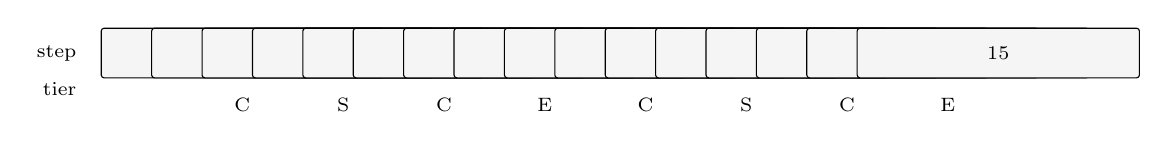
\begin{tikzpicture}[font=\scriptsize, x=6.4mm, y=7mm]
  \foreach \i in {0,...,15} {
    \draw[rounded corners=1pt, fill=black!4] (\i,0) rectangle ++(5.6,0.9);
    \node at (\i+2.8,0.45) {\i};
  }
  \foreach \i/\t in {0/C,2/S,4/C,6/E,8/C,10/S,12/C,14/E} {
    \node[below] at (\i+2.8,-0.2) {\t};
  }
  \node[left] at (-0.3,0.45) {step};
  \node[left] at (-0.3,-0.2) {tier};
\end{tikzpicture}
\end{center}

The C/S/E marks merely indicate tier 0/1/2; they are not the actual pattern of any style. Tier is the "skeleton / standard / fill" layer: complexity below 34 takes only tier 0; 34–66 takes tiers 0+1; 67 and above takes all three and lets the snare add low-velocity ghost notes in empty steps next to a primary hit, using a seed hash. Higher complexity means denser, not a different style.

Intensity does not change tiers, only velocity: the factor is $0.55 + 0.45 \times$ intensity/100. Intensity 100 equals the preset's original velocity; intensity 0 compresses it to 55%. Swing is in per-mille: 500 is straight, and larger values delay every odd sixteenth step more. The UI accepts 500–700; the generation core itself accepts 500–1000. Ratchet divides one step into up to 8 sub-hits, with sub-hit velocity scaled by $0.85 + 0.15 \times k/n$; it is not "retrigger the same step", but multiple onsets inside one step.

Fill only takes effect when "fill requested, preset has fill, and total bars $\geq$ 2": the last bar is replaced entirely by the fill lane table, and lanes absent from fill rest in that bar. Melodic lanes may carry an optional fourth element, pitch, but only for cowbell and 808 lanes; generation writes it as a constant pitch-bend curve, not per-sub-hit transposition.

Determinism is a hard contract: same style, same parameters, same seed $\Rightarrow$ byte-identical clip. The only random source is ghost-note decision, a pure hash of seed, GM key, and global step; it reads no clock and no global state.

\section{Drum presets and what generation produces}

There are 14 factory style presets compiled into the program and listed by the UI in fixed order; there is no "import style file" or "save custom style" entry. A style is not "a loop"; it is a recipe containing drum lanes, tiers, ratchets, layers, fill, per-lane chains, effects, and bus.

When generating a new drum track, Yeban does the following:

\begin{enumerate}
  \item Create a track named "<preset> Drums" at −6 dB, routed to the master bus. If the preset has a drum bus, first create an \texttt{AuxReturn} drum bus with glue compression and Soft Clipper; the drum track feeds the bus, and the bus feeds the master.
  \item If the target track has no source yet, install the default kit by family: acoustic binds the Virtuosity basic SFZ; electronic inserts a synth drum machine. An existing source is left alone; the user's kit wins.
  \item Append the preset's \texttt{fx} layer: channel strip and reverb are the base; some styles also carry tape, delay, transient shaping, bit crushing, or noise. Do not duplicate an existing non-bypassed effect of the same family; user effects win.
  \item Write the preset's \texttt{lane\_chains}; existing user lane chains are not overwritten.
  \item Write the preset's \texttt{automation}; an existing user lane for the same target is skipped.
  \item Add a MIDI clip and placement: from tick 0, length = bars × ticks per bar.
\end{enumerate}

If the current selection is a MIDI track (and not the master bus), generation lands on it; if the selection is an audio track, aux track, master bus, or nothing, a new drum track is created. Only the new-track path creates a drum bus; an existing track keeps its routing and gets no new bus.

\begin{center}
\begin{tikzpicture}[font=\scriptsize, >=latex, node distance=4mm]
  \node[draw, rounded corners, minimum width=19mm, minimum height=7mm] (style) {style preset};
  \node[draw, rounded corners, right=of style, minimum width=18mm, minimum height=7mm, align=center] (gen) {generator\\3 knobs + seed};
  \node[draw, rounded corners, right=of gen, minimum width=17mm, minimum height=7mm] (clip) {MIDI clip};
  \node[draw, rounded corners, below=of clip, minimum width=17mm, minimum height=7mm] (kit) {drum kit};
  \node[draw, rounded corners, left=of kit, minimum width=18mm, minimum height=7mm, align=center] (fx) {strip/reverb\\optional FX};
  \node[draw, rounded corners, left=of fx, minimum width=16mm, minimum height=7mm, align=center] (bus) {drum bus\\glue/clipper};
  \draw[->] (style) -- (gen);
  \draw[->] (gen) -- (clip);
  \draw[->] (gen) -- (kit);
  \draw[->] (kit) -- (fx);
  \draw[->] (fx) -- (bus);
\end{tikzpicture}
\end{center}

\section{Using the dialog}

The entry is "Edit → Drum Generation (Drums)...". The dialog's left column lists the 14 styles; the right column has five text fields, a last-bar fill toggle, a target-track line, and a "Generate" button.

\begin{table}[htbp]
\centering
\small
\begin{tabular}{@{}llll@{}}
\hline
Control & Meaning & Range & Default \\
\hline
Style & Factory preset, choose one & 14 items & first item \\
Complexity & Density/layers & 0–100 & 50 \\
Intensity & Velocity scaling & 0–100 & 80 \\
Swing & Odd-sixteenth delay (per-mille) & UI 500–700 & preset value \\
Bars & Generated length & 1–16 & 4 \\
Base seed & Salt for ghost-note hash & u64 & project seed \\
Last-bar fill & Replace last bar with fill & on/off & on \\
\hline
\end{tabular}
\caption{Controls in the drum generation dialog}
\label{tab:drum-dialog}
\end{table}

Picking a style seeds the swing field with that style's fixed value; blank complexity, intensity, and bars seed as 50, 80, and 4; a blank seed uses the project seed. Parse failure leaves the dialog open, writes the reason in the error line, and submits nothing. Generating twice with the same style and parameters produces byte-identical clip content.

\screenshot{drum-gen-dialog}{The "Drum Generation" dialog is open: style list on the left, complexity/intensity/swing/bars/seed/fill on the right, target-track line and "Generate" button at the bottom.}

\screenshot{drum-track-device-rack}{The generated electronic drum track in the device rack shows the synth drum machine, channel strip, reverb, and optional delay; parameters are read-only.}

\screenshot{drum-clip-piano-roll}{The generated drum clip appears as a column of MIDI notes in the piano roll, editable by key and velocity.}

\section{What Yeban does not have}

\begin{itemize}
  \item \textbf{No 16-step editor.} Drum generation is "template + rule transformation", not a grid you light step by step; the generated MIDI clip can be edited in the arrangement and piano roll, but there is no dedicated drum-step grid.
  \item \textbf{No save entry for custom kits/styles.} The 14 styles are factory read-only; the device card shows drum parameters but cannot turn kick tune or snare decay.
  \item \textbf{No 808/909 circuit modeling.} The 13 voices are synthesis recipes; "808/909" is a parameter-level recipe, not transistor-level analog modeling, and there is no component spread.
  \item \textbf{No per-voice independent outputs, per-voice sends, or parallel compression.} The drum machine is a summed output (with per-voice pan), not a box with separate outputs.
  \item \textbf{No second choke group.} Only closed hat chokes open hat; crash, toms, and others have no choke.
  \item \textbf{No second synth drum machine on the same track.} One track, one source; to layer acoustic and electronic, use two tracks.
\end{itemize}

\section{Help-topic mapping}

\begin{table}[htbp]
\centering
\small
\begin{tabular}{@{}p{0.40\linewidth}p{0.48\linewidth}@{}}
\hline
Section & In-app help anchor \\
\hline
Two timbre routes & \texttt{drum-families} \\
How the drum timbres are synthesized & \texttt{drum-voice-synthesis} \\
Step sequencing & \texttt{drum-step-sequencing} \\
Drum presets and what generation produces & \texttt{drum-presets-generation} \\
Using the dialog & \texttt{drum-dialog} \\
What Yeban does not have & \texttt{drum-current-limits} \\
\hline
\end{tabular}
\caption{Help-topic mapping for Chapter 6}
\end{table}
